% --- SLIDES : Challenge 1 ---

\section{Challenge Diffie-Hellman}

\begin{frame}
    \frametitle{Diffie-Hellman : \textit{Man-in-the-middle | Export grade}}
    \framesubtitle{Objectifs}
    \begin{center}
        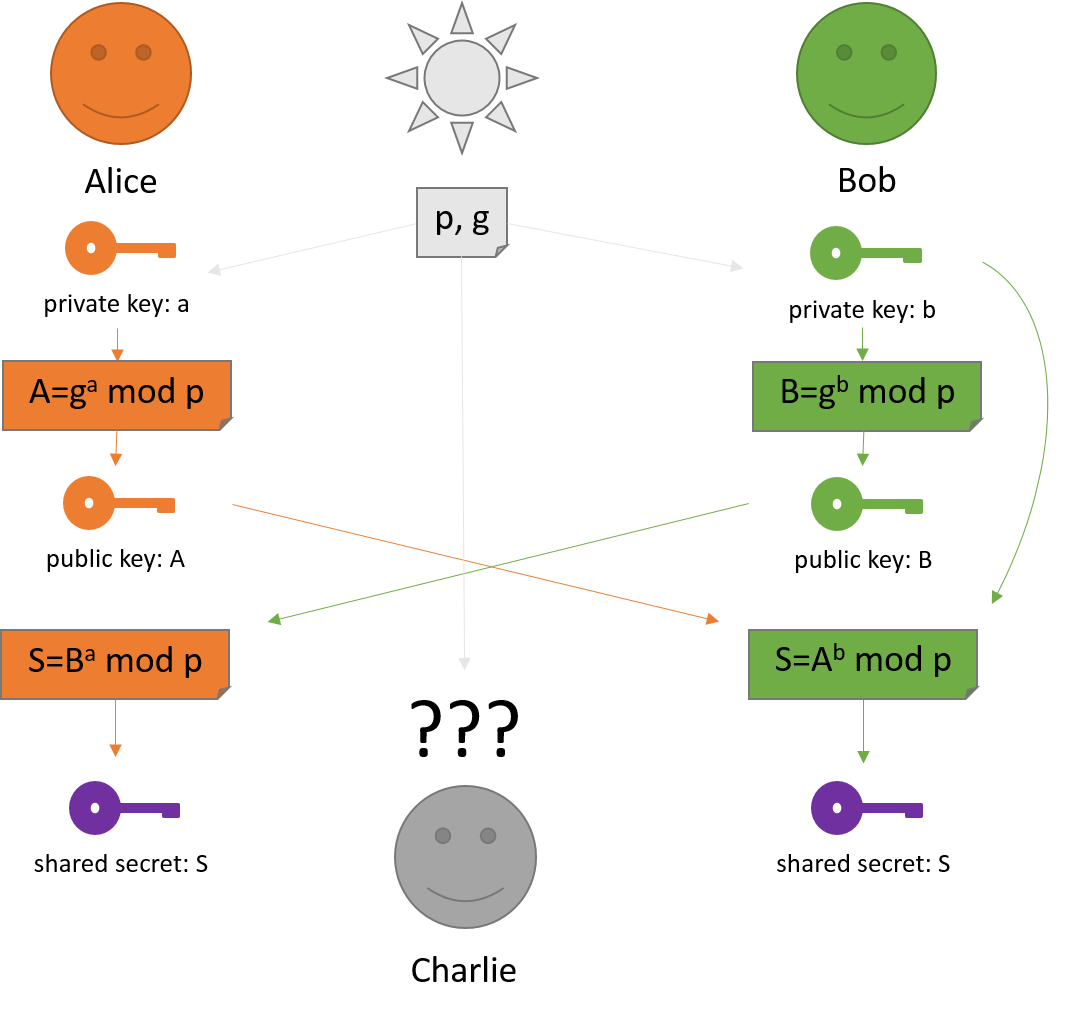
\includegraphics[width=0.65\textwidth]{diffie_key_exchange.png}
        \vspace{0.5em}
    \end{center}
\end{frame}

\begin{frame}
    \frametitle{Diffie-Hellman : \textit{Man-in-the-middle | Export grade}}
    \framesubtitle{Méthode de résolution}
    \begin{center}
        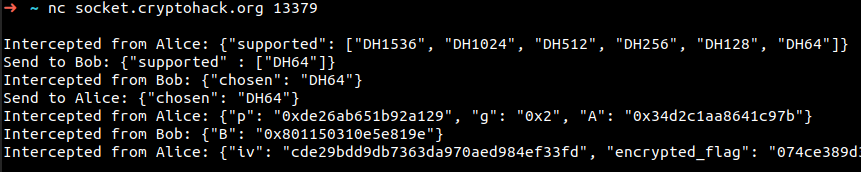
\includegraphics[width=1\textwidth,trim=0 5cm 0 0,clip]{screen_export_grade.png}
        \vspace{0.5em}
    \end{center}
\end{frame}

\begin{frame}
    \frametitle{Diffie-Hellman : \textit{Man-in-the-middle | Export grade}}
    \framesubtitle{Méthode de résolution}
    \begin{center}
        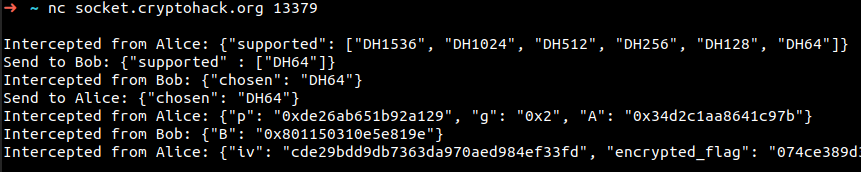
\includegraphics[width=1\textwidth,trim=0 3.5cm 0 0,clip]{screen_export_grade.png}
        \vspace{0.5em}
    \end{center}
\end{frame}

\begin{frame}
    \frametitle{Diffie-Hellman : \textit{Man-in-the-middle | Export grade}}
    \framesubtitle{Méthode de résolution}
    \begin{center}
        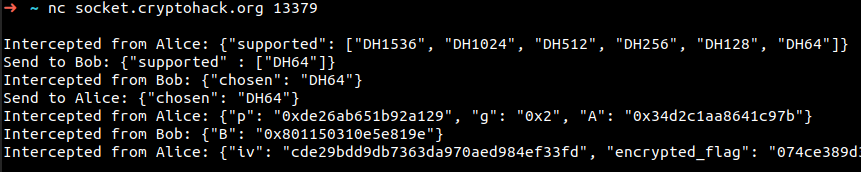
\includegraphics[width=1\textwidth,trim=0 2.2cm 0 0,clip]{screen_export_grade.png}
        \vspace{0.5em}
    \end{center}
\end{frame}

\begin{frame}
    \frametitle{Diffie-Hellman : \textit{Man-in-the-middle | Export grade}}
    \framesubtitle{Méthode de résolution}
    \begin{center}
        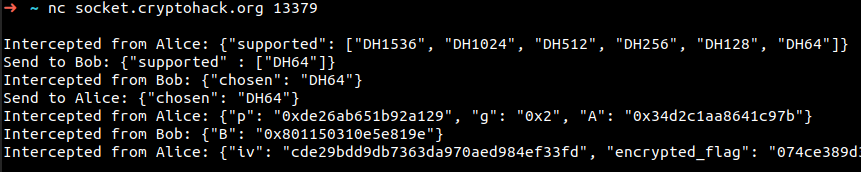
\includegraphics[width=1\textwidth]{screen_export_grade.png}
        \vspace{0.5em}
    \end{center}
\end{frame}

\begin{frame}
    \frametitle{Diffie-Hellman : \textit{Man-in-the-middle | Export grade}}
    \framesubtitle{Méthode de résolution}

    \begin{figure}
        \centering
        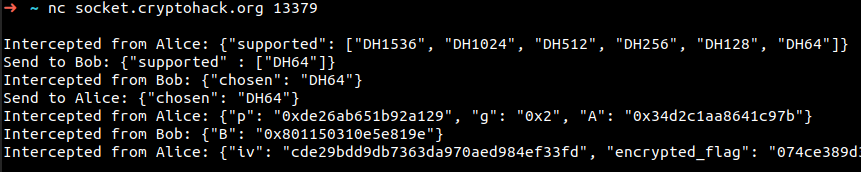
\includegraphics[width=0.9\textwidth]{screen_export_grade.png}
    \end{figure}

    \begin{block}{Étapes clés de l'attaque}
        \begin{itemize}
            \item Attaque de type \textit{Man-in-the-middle} pour manipuler la communication.
            \item Forcer Alice et Bob à utiliser un \textbf{paramètre de sécurité faible} (64 bits).
            \item La faiblesse du paramètre rend la résolution du \textbf{logarithme discret} possible, ce qui nous donne accès au secret partagé.
        \end{itemize}
    \end{block}
    
\end{frame}


\begin{frame}
    \frametitle{Diffie-Hellman : \textit{Man-in-the-middle | Export grade}}
    \framesubtitle{Résultat}

    \begin{block}{Calcul de la clé secrète partagée}
        Grâce aux paramètres faibles, nous pouvons résoudre le logarithme discret pour trouver la clé privée d'Alice ($a$) :
        $$ a = \log_g(A) \pmod{p} $$
        
        Puis, nous utilisons cette clé privée pour calculer le secret partagé ($s$) avec la clé publique de Bob ($B$) :
        $$ s = B^a \pmod{p} $$
    \end{block}
    
    \vspace{1em}
    
    Une fois le secret partagé \textit{s} obtenu, il ne reste plus qu'à dériver la clé pour obtenir le flag : 

        \begin{center}
            \Large\texttt{crypto\{d0wn6r4d35\_4r3\_d4n63r0u5\}}
        \end{center}

\end{frame}